\documentclass{beamer}
\usepackage{pgfplots}
\usepackage[utf8]{inputenc}
\usepackage[T1]{fontenc}
\usepackage{pgfplots}
\pgfplotsset{width=10cm,compat=1.9}

\title{Introduction to pgfplots}
\author{Martin Maina}
\institute{JKUAT}
\date{\today}

\begin{document}

\begin{frame}
  \titlepage
\end{frame}

\begin{frame}{Introduction}
  The \texttt{pgfplots} package, based on TikZ, is a powerful tool for creating scientific/technical graphics. It simplifies the process by allowing you to provide the input data or formula, and \texttt{pgfplots} takes care of the rest.
\end{frame}
\begin{frame}{Document Preamble}
  To use \texttt{pgfplots} in your document, add the following line to your preamble:
  
  \texttt{\textbackslash usepackage\{pgfplots\}}
  
  You can also configure the behavior of \texttt{pgfplots} in the preamble. For example, to change the size of each plot and ensure backward compatibility, add the following line:
  
  \texttt{\textbackslash pgfplotsset\{width=10cm,compat=1.9\}}
  
  This sets the size of each \texttt{pgfplots} figure to 10 centimeters. You can use different units such as pt, mm, or in.
\end{frame}

\begin{frame}{Compilation Time}
  When the original TeX engine was created, it wasn't designed for direct production of graphics. The introduction of pdfTeX allowed for direct graphics creation using built-in TeX language commands. This led to the development of LaTeX graphics packages like TikZ and \texttt{pgfplots}.
  
  However, the processing of high-level LaTeX graphics commands into low-level pdfTeX commands can take time. Documents with multiple \texttt{pgfplots} figures or complex graphics may have longer compilation times.
\end{frame}

\begin{frame}{Reducing Compilation Time}
  To increase the speed of document compilation, you can configure \texttt{pgfplots} to export the figures to separate PDF files and then import them into the document. This allows you to compile once and reuse the figures.
  
  To enable this, add the following code to the preamble:
  
  \texttt{\textbackslash usepgfplotslibrary\{external\}}
  
  \texttt{\textbackslash tikzexternalize}
\end{frame}

\begin{frame}{Basic Example (Externalizing Figures)}
\begin{figure}
  \centering
  % Here begins the 2D plot
  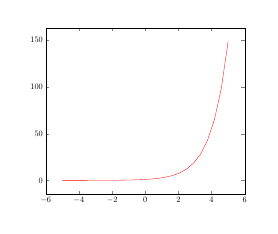
\begin{tikzpicture}[scale=0.3]
    \begin{axis}
      \addplot[color=red]{exp(x)};
    \end{axis}
  \end{tikzpicture}
  % Here ends the 2D plot
  \hskip 5pt
  % Here begins the 3D plot
  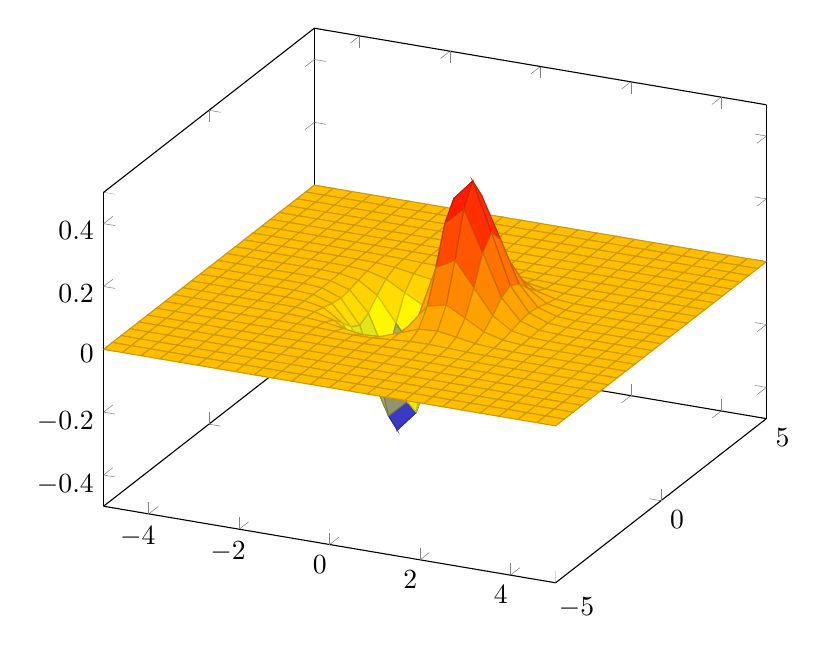
\begin{tikzpicture}
    \begin{axis}
      \addplot3[surf]{exp(-x^2-y^2)*x};
    \end{axis}
  \end{tikzpicture}
  % Here ends the 3D plot
  \caption{2D and 3D math expressions plotted side-by-side.}
\end{figure}
\end{frame}

\begin{frame}[fragile]
  \frametitle{Plotting from Data: Explanation}

  \begin{itemize}
    \item The code snippet demonstrates how to plot data with \texttt{pgfplots}.
    \item The plot showcases the temperature dependence of CuSO\(_4\cdot\)5H\(_2\)O solubility.
    \item The \texttt{title} command sets the title of the plot.
    \item The \texttt{xlabel} and \texttt{ylabel} specify the labels for the x-axis and y-axis, respectively.
    \item The \texttt{xmin}, \texttt{xmax}, \texttt{ymin}, and \texttt{ymax} options define the range of the x-axis and y-axis.
    \item The \texttt{xtick} and \texttt{ytick} parameters determine the tick positions on the x-axis and y-axis.
    \item The \texttt{legend pos} sets the position of the legend box (northwest in this case)
  \end{itemize}

\end{frame}

\begin{frame}[fragile]
  \frametitle{Plotting from Data: Explanation}
  \begin{itemize}
   \item \texttt{ymajorgrids} enables the grid lines on the y-axis, and \texttt{grid style} determines their style.
    \item The \texttt{color} option sets the color of the plotted line, and \texttt{mark} specifies the shape of the data points (squares in this case).
    \item The \texttt{coordinates} section contains the data points to be plotted.
    \item The \texttt{\textbackslash legend} command adds a legend entry for the plot.
  \end{itemize}
  This example demonstrates how to plot data from coordinates using \texttt{pgfplots}. It provides a clear visual representation of the temperature dependence of CuSO\(_4\cdot\)5H\(_2\)O solubility.
\end{frame}

\begin{frame}{2D Plots}
\begin{figure}
  \centering
  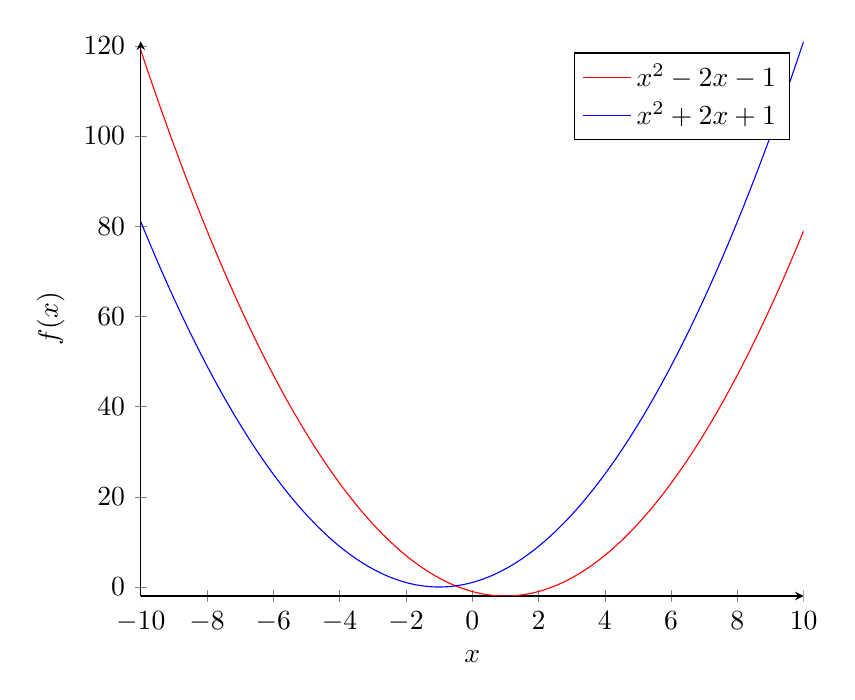
\begin{tikzpicture}
    \begin{axis}[
      axis lines = left,
      xlabel = \(x\),
      ylabel = {\(f(x)\)},
    ]
    % Below the red parabola is defined
    \addplot [
      domain=-10:10,
      samples=100,
      color=red,
    ]{x^2 - 2*x - 1};
    \addlegendentry{\(x^2 - 2x - 1\)}
    % Here the blue parabola is defined
    \addplot [
      domain=-10:10,
      samples=100,
      color=blue,
    ]{x^2 + 2*x + 1};
    \addlegendentry{\(x^2 + 2x + 1\)}
    \end{axis}
  \end{tikzpicture}
  \caption{Plotting mathematical expressions.}
\end{figure}
\end{frame}

\begin{frame}[fragile]
  \frametitle{Plotting from Data}
  
  \begin{verbatim}
\begin{figure}
  \centering
  \begin{tikzpicture}
    \begin{axis}[
      title={Temperature dependence of
 CuSO\(_4\cdot\)5H\(_2\)O solubility},
      xlabel={Temperature [\textcelsius]},
      ylabel={Solubility [g per 100 g water]},
      xmin=0, xmax=100,
      ymin=0, ymax=120,
      xtick={0,20,40,60,80,100},
      ytick={0,20,40,60,80,100,120},
      legend pos=north west,
      ymajorgrids=true,
      grid style=dashed,
    ]
\end{figure}
  \end{verbatim}
\end{frame}

\begin{frame}[fragile]
\begin{verbatim}
	\begin{figure}
	\centering
 \addplot[
      color=blue,
      mark=square,
    ]
    coordinates {
      (0,23.1)(10,27.5)(20,32)(30,37.8)
(40,44.6)(60,61.8)(80,83.8)(100,114)
    };
    \legend{CuSO\(_4\cdot\)5H\(_2\)O}
    
    \end{axis}
  \end{tikzpicture}
  \caption{Temperature dependence of 
CuSO\(_4\cdot\)5H\(_2\)O solubility}
\end{figure}
  \end{verbatim}
\end{frame}
\begin{frame}
  \frametitle{Plotting from Data: Explanation}

  \begin{itemize}
    \item The code snippet demonstrates how to plot data with `pgfplots`.
    \item The plot showcases the temperature dependence of CuSO\(_4\cdot\)5H\(_2\)O solubility.
    \item The `title` command sets the title of the plot.
    \item The `xlabel` and `ylabel` specify the labels for the x-axis and y-axis, respectively.
    \item The `xmin`, `xmax`, `ymin`, and `ymax` options define the range of the x-axis and y-axis.
    \item The `xtick` and `ytick` parameters determine the tick positions on the x-axis and y-axis.
    \item The `legend pos` sets the position of the legend box (northwest in this case).
    \item `ymajorgrids` enables the grid lines on the y-axis, and `grid style` determines their style
  \end{itemize}
\end{frame}

\begin{frame}[fragile]
\begin{itemize}
 \item `ymajorgrids` enables the grid lines on the y-axis, and `grid style` determines their style.
    \item The `color` option sets the color of the plotted line, and `mark` specifies the shape of the data points (squares in this case).
    \item The `coordinates` section contains the data points to be plotted.
    \item The \texttt{\textbackslash legend} command adds a legend entry for the plot.
  \end{itemize}
  This example demonstrates how to plot data from coordinates using `pgfplots`. It provides a clear visual representation of the temperature dependence of CuSO\(_4\cdot\)5H\(_2\)O solubility.
\end{frame}


%\begin{frame}[fragile]
%  \frametitle{3D Plots: Plotting Mathematical Expressions}
%
%  \begin{columns}[T]
%    \begin{column}{0.6\textwidth}
%      \begin{itemize}
%        \item The code snippet demonstrates plotting a mathematical expression in 3D using \texttt{pgfplots}.
%        \item The plot showcases the usage of the \texttt{mesh} parameter.
%        \item The \texttt{hide axis} option hides the axes.
%        \item The \texttt{colormap/cool} sets the color scheme for the plot.
%        \item The \texttt{addplot3} command adds the plot to the axis.
%        \item The \texttt{samples} parameter determines the number of samples.
%        \item The \texttt{domain} specifies the domain of the function.
%      \end{itemize}
%    \end{column}
%    \begin{column}{0.4\textwidth}
%      \begin{center}
%        \includegraphics[width=\textwidth]{Pgfplots3dexample.png}
%      \end{center}
%    \end{column}
%  \end{columns}
%\end{frame}
%
%\begin{frame}[fragile]
%  \frametitle{3D Plots: Contour Plots}
%
%  \begin{columns}[T]
%    \begin{column}{0.6\textwidth}
%      \begin{itemize}
%        \item The code snippet demonstrates plotting contour plots in 3D using \texttt{pgfplots}.
%        \item The plot showcases the usage of the \texttt{contour gnuplot} parameter.
%        \item The \texttt{view} parameter controls the viewing angle of the plot.
%        \item The \texttt{levels} parameter sets the contour levels.
%      \end{itemize}
%    \end{column}
%    \begin{column}{0.4\textwidth}
%      \begin{center}
%       % \includegraphics[width=\textwidth]{Contourplotexample.png}
%      \end{center}
%    \end{column}
%  \end{columns}
%\end{frame}

\begin{frame}{3D Plots}
    pgfplots has the 3D Plotting capabilities that you may expect in a plotting software.
\end{frame}

\begin{frame}{Plotting mathematical expressions}
    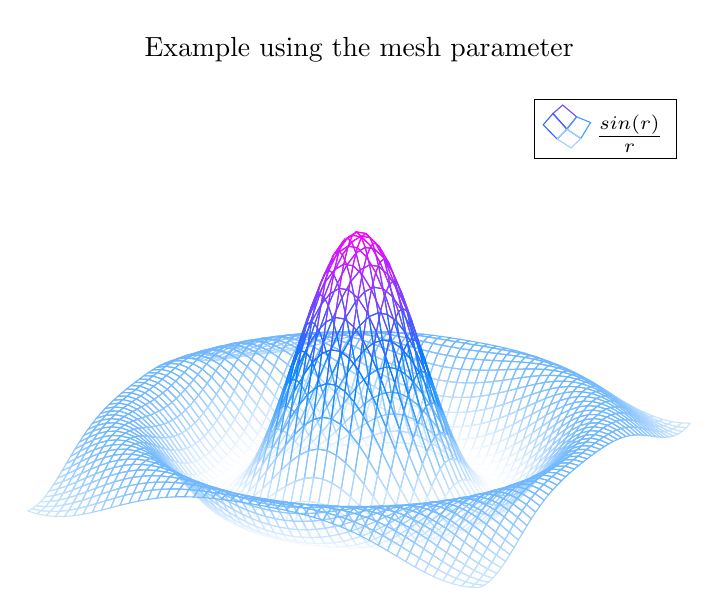
\begin{tikzpicture}
        \begin{axis}[
            title=Example using the mesh parameter,
            hide axis,
            colormap/cool,
        ]
        \addplot3[
            mesh,
            samples=50,
            domain=-8:8,
        ]
        {sin(deg(sqrt(x^2+y^2)))/sqrt(x^2+y^2)};
        \addlegendentry{\(\frac{sin(r)}{r}\)}
        \end{axis}
    \end{tikzpicture}
    When working with trigonometric functions pgfplots uses degrees as default units, if the angle is in radians (as in this example) you have to use the deg function to convert to degrees.
\end{frame}

\begin{frame}{Contour plots}
%\begin{verbatim}
%    \begin{tikzpicture}
%        \begin{axis}
%        [
%            title={Contour plot, view from top},
%            view={0}{90}
%        ]
%        \addplot3[
%            contour gnuplot={levels={0.8, 0.4, 0.2, -0.2}}
%        ]
%        {sin(deg(sqrt(x^2+y^2)))/sqrt(x^2+y^2)};
%        \end{axis}
%    \end{tikzpicture}
%    \end{verbatim}
    \begin{itemize}
        \item The value of the title parameter is inside curly brackets because it contains a comma, so we use the grouping brackets to avoid any confusion with the other parameters passed to the \texttt{\textbackslash begin\{axis\}} declaration.
        \item \texttt{view=\{0\}\{90\}} changes the view of the plot. The first value is a rotation, in degrees, around the z-axis; the second value is to rotate the view around the x-axis. In this example when we combine a 0° rotation around the z-axis and a 90° rotation around the x-axis we end up with a view of the plot from top.
        \item \texttt{contour gnuplot=\{levels=\{0.8, 0.4, 0.2, -0.2\}\}} tells LaTeX to use the external software gnuplot to compute the contour lines; this works fine in Overleaf but if you want to use this command in your local LaTeX installation you have to install gnuplot first (matlab will also work, in such case write matlab instead of gnuplot in the command). The sub parameter levels is a list of values of elevation levels where the contour lines are to be computed.
    \end{itemize}
\end{frame}
		
		\begin{frame}{Plotting a surface from data}
		    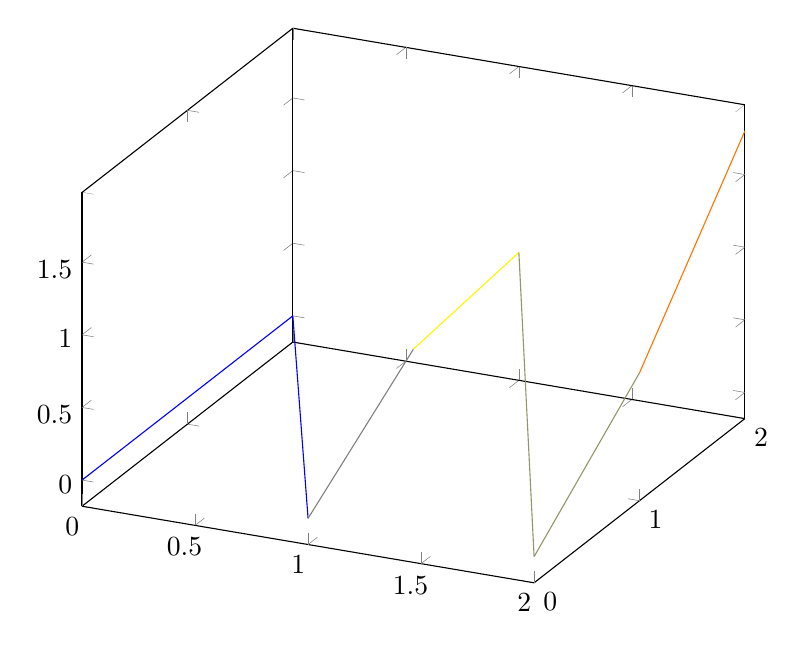
\begin{tikzpicture}
		        \begin{axis}
		        \addplot3[
		            surf,
		        ] 
		        coordinates {        (0,0,0) (0,1,0) (0,2,0)        (1,0,0) (1,1,0.6) (1,2,0.7)                        (2,0,0) (2,1,0.7) (2,2,1.8)        };
		        \end{axis}
		    \end{tikzpicture}
		    
		    The points passed to the \texttt{coordinates} parameter are treated as contained in a $3 \times 3$ matrix, using a blank line as the separator for each matrix row.
		
		    All the options for 3D plots in this article apply to data surfaces.
		    
		\end{frame}

\begin{frame}{Parametric plot}
    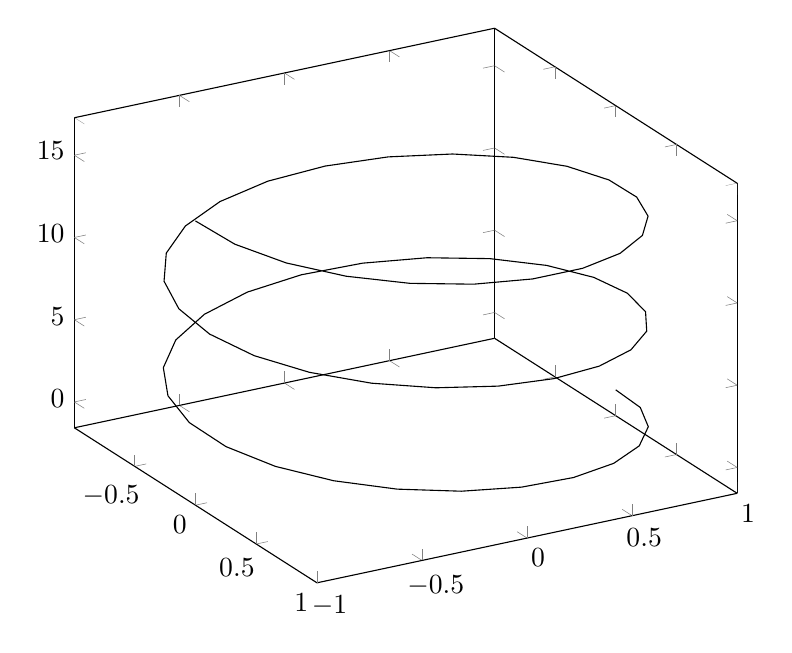
\begin{tikzpicture}
        \begin{axis}[
            view={60}{30},
        ]
        \addplot3[
            domain=0:5*pi,
            samples=60,
            samples y=0,
        ]
        ({sin(deg(x))}, {cos(deg(x))}, {x});
        \end{axis}
    \end{tikzpicture}
   
    \begin{itemize}
        \item \texttt{samples y=0} is used to prevent pgfplots from joining the extreme points of the spiral.
        \item The function to plot is passed to the \texttt{addplot3} environment. Each parameter function is grouped inside curly brackets and the three parameters are delimited with parentheses.
    \end{itemize}
    
\end{frame}

\end{document}

\end{document}
